%
% $Id: slides.tex 4228 2006-06-21 21:55:12Z jjamor $
%
%
% Compilar a .pdf con LaTeX (pdflatex)
% Es necesario instalar Beamer (paquete latex-beamer en Debian)
%

%
% Gráficos:
% Los gráficos pueden suministrarse en PNG, JPG, TIF, PDF, MPS
% Los EPS deben convertirse a PDF (usar epstopdf)
%

\documentclass{beamer}
\usetheme{Warsaw}
\usebackgroundtemplate{
\includegraphics[width=\paperwidth]{format/opensistemas-bg.png}}
\usepackage[spanish]{babel}
\usepackage[latin1]{inputenc}
\usepackage{hyperref}
\usepackage{graphics}
\usepackage{amssymb} % Simbolos matematicos

%\definecolor{libresoftgreen}{RGB}{162,190,43}
%\definecolor{libresoftblue}{RGB}{0,98,143}

%\setbeamercolor{titlelike}{bg=libresoftgreen}

%% Metadatos del PDF.
\hypersetup{
  pdftitle={Introduction to Solaris LDOMs},
  pdfauthor={Juanjo Amor},
  pdfcreator={OpenSistemas},
  pdfproducer=PDFLaTeX,
  pdfsubject={Open Source},
}
%%

\AtBeginSection[]
{
  \begin{frame}<presentation>
    \frametitle{Index}
    \tableofcontents[current]
  \end{frame}
}


\begin{document}

%%\renewcommand{\pause}{}

\title{Solaris LDOMs}
\subtitle{Hypervisor-based virtualization for Sparc T}
\institute{jjamor@opensistemas.com\\
OpenSistemas}
\author{Juanjo Amor}
\date{27 May 2011}

\frame{
\maketitle
\begin{center}

\includegraphics[width=6cm]{format/gsyc-open-urjc}
\end{center}
}


% Si el titulo o el autor se quieren acortar para los pies de página
% se pueden redefinir aquí:
%\title{Titulo corto}
%\author{Autores abreviado}


%% LICENCIA DE REDISTRIBUCION DE LAS TRANSPAS
\frame{
~
\vspace{4cm}

\begin{flushright}
{\tiny
(cc) 2011 Juanjo Amor\\
  Some rights reserved. This work licensed under Creative Commons\\
  Attribution-ShareAlike License. To view a copy of full license, see\\
  http://creativecommons.org/licenses/by-sa/3.0/ or write to\\
  Creative Commons, 559 Nathan Abbott Way, Stanford,\\
  California 94305, USA.\\

%  Este documento (o uno muy similar) está disponible en \\
%  \url{http://gsyc.escet.urjc.es/~jjamor/}
}
\end{flushright}
}
%%

\section{About Opensistemas}

%%%%%%%%%%%%%%%%%%%%%%%%%%%%%%%%%%%%%%%%%%%%%%%%%%%%%%%%%%%%%%

\begin{frame}
\frametitle{About Opensistemas}
\begin{center}
Opensistemas is an {\LARGE international} company \pause highly {\LARGE specialized} \pause in
offering global {\Huge IT solutions} \pause based on {\Huge Open Source} and {\Huge Linux} platforms.
\end{center}
\end{frame}

\begin{frame}
\frametitle{About Opensistemas}
\begin{itemize}
\item Our Vision:
\pause
To become the international leader in Open Source Technologies.
\pause
\item Our Mission:
\pause
Apply our knowledge of the opportunities offered by Open Source to deliver
effective solutions and innovation to our customers while promoting the
professional development of our employees and building value for 
shareholders.
\pause
\item Our Values:
\pause
\begin{itemize}
\item Deliver effective solutiosn to our customers.
\item Corporate social responsibility.
\item Commitment to Open Source.
\item Ethics and Respect for individuals.
\item Research and Innovation.
\item Teamwork.
\item Commitment to the development of a society connected by information
and knowledge.
\end{itemize}
\end{itemize}
\end{frame}

\begin{frame}
\frametitle{About Opensistemas}
\begin{center}
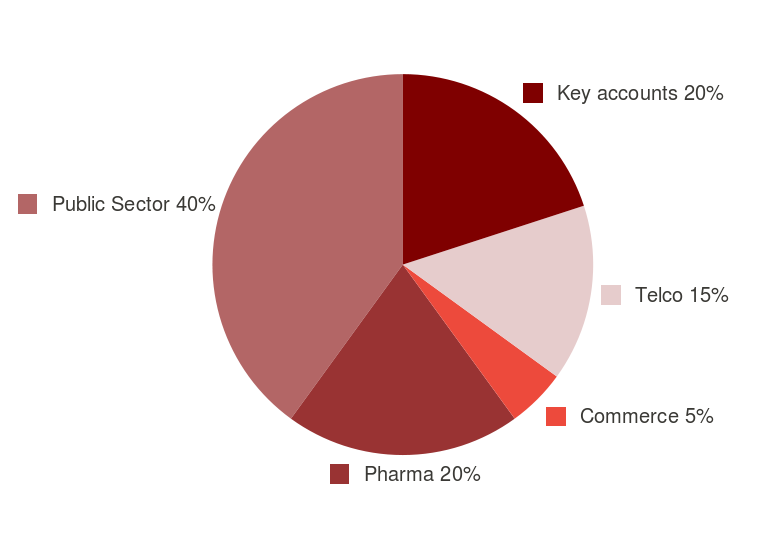
\includegraphics[width=9cm]{figs/opensistemas-markets}
\end{center}
\begin{center}
Our Markets
\end{center}
\end{frame}

\begin{frame}
\frametitle{About Opensistemas}
\begin{center}
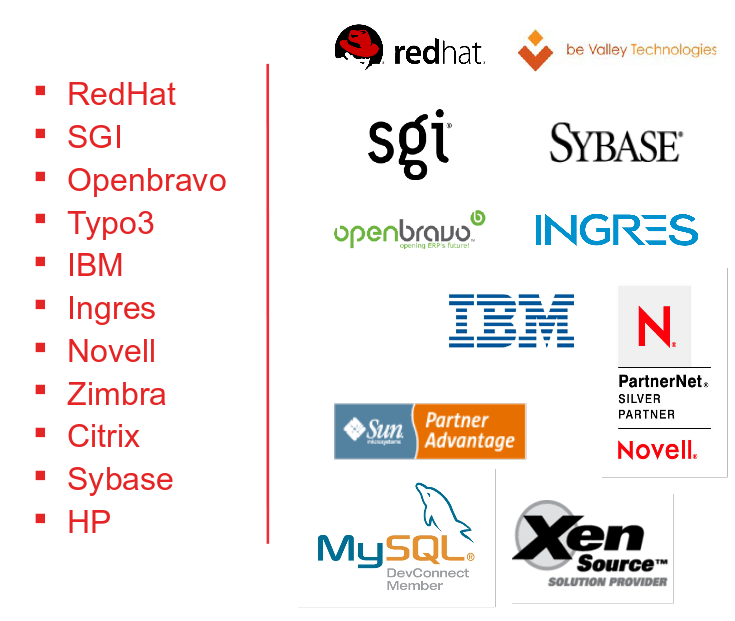
\includegraphics[width=7cm]{figs/opensistemas-partners}
\end{center}
\begin{center}
Our Partners
\end{center}
\end{frame}

\begin{frame}

\frametitle{About Opensistemas}
\begin{center}
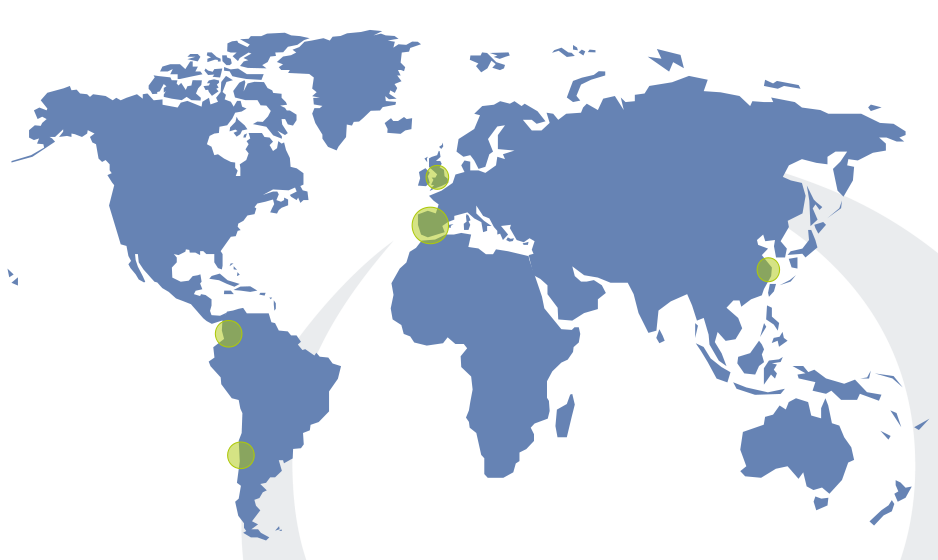
\includegraphics[width=9cm]{figs/opensistemas-worldmap}
\end{center}
\begin{center}
{\small Opensistemas is present in nine locations over five countries: Spain (Madrid, Valencia, Barcelona, Sevilla, Zaragoza), Chile (Santiago), Colombia (Bogotá), United Kingdom (London) and China (Shanghai).}
\end{center}
\end{frame}

\begin{frame}

\frametitle{About Opensistemas}
{\Huge Contact Information}
\begin{itemize}
\item \textcolor{blue}{\url{http://www.opensistemas.com/}}
\item info@opensistemas.com
\item +34 902 107 396
\end{itemize}
\end{frame}

\section{LDOMs}

\begin{frame}
\frametitle{Oracle VM projects}

\begin{itemize}
\item Virtualbox: \pause VMs for all. Cross-platform.\pause
\item VM server for x86: \pause Xen ported to Solaris/Illumos x86, and for Oracle Linux.\pause
\item VM Server for Sparc (formerly LDOMs): \pause Type I hypervisor, ``full'', for Sparc T platform.\pause
\item Zones: \pause Light virtualization for Solaris/Illumos.\pause
\item Other: \pause Ops center, VDI\ldots
\end{itemize}

\end{frame}

\begin{frame}
\frametitle{What are LDOMs?}

LDOMs (Oracle VM Server for Sparc) are {\em Logical Domains}:
\pause
\begin{itemize}
\item Hypervisor for (Open)Solaris running in specific hardware.
\pause
\item Type I hypervisor: layer between hardware and all OS.
\pause
\item LDOMs hypervisor is run by the server firmware...
\pause
\item ... and one of the guest OS have special privileges to manage hypervisor (``control domain'')
\end{itemize}

\end{frame}

\begin{frame}
\frametitle{What are LDOMs?}

LDOMs:
\pause
\begin{itemize}
\item ``full virtualization'', type I hypervisor\pause
\item It requires special CPUs (Chip Multithreading = CMT).\pause
\item Base OS: Solaris 10 / 11 / Opensolaris 2009.06\pause
\item Guest OS:\pause
\begin{itemize}
\item Solaris 10/11, Opensolaris 2009.06, Illumos?\pause
\item Sparc Linux and other OS which support this architecture.\pause
\end{itemize}
\item Currently, only SunOS is supported as Guest OS.
\end{itemize}

\end{frame}

\begin{frame}
\frametitle{Chip Multithreading (CMT)}


\begin{itemize}
\item Ultrasparc T1/T2/T3\pause
\item Multithread. A thread is similar to a CPU.\pause
\begin{itemize}
\item Example: T1 has 8 cores with 4 threads/core.\pause
\end{itemize}
\item Direct SSL support on hardware (1 MAU/core).\pause
\item LDOMs can assign threads to VMs.\pause
\item Hypervisor runs on server firmware.\pause
\item ``free'' hardware: \textcolor{red}{\url{http://www.opensparc.net/}}\pause
\item Sun Fire T / Enterprise T / Blade T Servers

\begin{flushright}
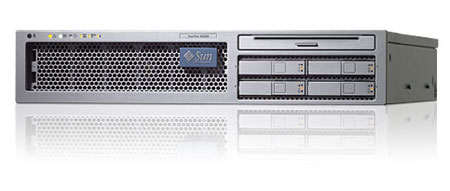
\includegraphics[width=6cm]{figs/sunT2000.jpg}
\end{flushright}

\end{itemize}


\end{frame}

\begin{frame}[fragile]
\frametitle{Installing LDOMs}

1. LDOMs 1.2 may require firmware upgrade:
\pause
\begin{itemize}
\item some servers could have firmware older than 6.7.4.
\end{itemize}

\pause

{\tiny
\begin{verbatim}
sc> showhost
Sun-Fire-T2000 System Firmware 6.5.3 2007/10/03 05:56

Host flash versions:
Hypervisor 1.5.2 2007/09/25 08:39
OBP 4.27.4 2007/10/02 18:35
POST 4.27.4 2007/10/02 19:03

# ./sysfwdownload ./Sun_System_Firmware-6_7_4-Sun_Fire_T2000.bin
... ... ... ...
Download completed succesfully.

sc> flashupdate -s 127.0.0.1
... ... ...
Update complete. Reset device to use new software.
sc> resetsc
\end{verbatim}
}

\end{frame}

\begin{frame}[fragile]
\frametitle{Installing LDOMs (II)}

2. Install ldoms manager 1.2 package.\pause
\begin{itemize}
\item Package available in Opensolaris repository.
\end{itemize}
\pause
{\tiny
\begin{verbatim}
# pkg install ldomsmanager
\end{verbatim}
}
\pause
3. Initial setup of {\em domain controller}.
\pause
{\tiny
\begin{verbatim}
global# ldm add-vds primary-vds0 primary
global# ldm add-vcc port-range=5000-5100 primary-vcc0 
global# ldm add-vsw net-dev=e1000g2 primary-vsw0 primary
global# ldm set-mau 1 primary
global# ldm set-vcpu 16 primary
global# ldm set-memory 16384m primary
global# ldm ls
------------------------------------------------------------------------------ 
Notice: the LDom Manager is running in configuration mode. Configuration and
resource information is displayed for the configuration under construction;
not the current active configuration. The configuration being constructed
will only take effect after it is downloaded to the system controller and
the host is reset.
------------------------------------------------------------------------------
NAME STATE FLAGS CONS VCPU MEMORY UTIL UPTIME
primary active -n-cv- SP 16 16G 0.0% 1h 9m
\end{verbatim}
}

\end{frame}

\begin{frame}[fragile]
\frametitle{Installing LDOMs (III)}

5. Load configuration to system controller (SC) and reboot.
\pause
{\tiny
\begin{verbatim}
global# ldm list-spconfig
factory-default [current]
global# ldm add-spconfig config_01
global# ldm list-spconfig
global# init 6
...
...
syncing file systems... done
rebooting...

SC Alert: Host System has Reset
...
...
Sun Fire T200, No Keyboard
Copyright 2009 Sun Microsystems, Inc.  All rights reserved.
OpenBoot 4.30.3, 16384 MB memory available, Serial #70066726.
Ethernet address 0:14:4f:2d:22:26, Host ID: 842d2226.
\end{verbatim}
}

\end{frame}

\begin{frame}[fragile]
\frametitle{Creating a LDOMs domain}

1. Create and start the domain.
\pause
{\tiny
\begin{verbatim}
global# ldm add-domain t2000-01
global# ldm add-vcpu 4 t2000-01
global# ldm add-memory 2048m t2000-01
global# mkfile 4G /export/ldomsvdisks/t2000-01-00.img 
global# ldm add-vdsdev /export/ldomsvdisks/t2000-01-00.img vol1@primary-vds0
global# ldm add-vdisk vdisk1 vol1@primary-vds0 t2000-01
global# ldm add-vdsdev /export/aiserver/solaris10-01.iso iso@primary-vds0
global# ldm add-vdisk vcdrom iso@primary-vds0 t2000-01
global# ldm add-vnet vnet1 primary-vsw0 t2000-01
global# ldm bind-domain t2000-01
global# ldm start-domain t2000-01
global# ldm ls
NAME STATE FLAGS CONS VCPU MEMORY UTIL UPTIME
primary active -n-cv- SP 16 16G 0.2% 1h 9m
t2000-01 active -t---- 5000 4 2G 25% 1m
\end{verbatim}
}
\pause
2. Enter the domain console.
\pause
{\tiny
\begin{verbatim}
global# telnet 127.0.0.1 5000

Connecting to console "t2000-01" in group "t2000-01" ....
Press ~? for control options ..

Sun Fire T200, No Keyboard
Copyright 2009 Sun Microsystems, Inc. All rights reserved.
OpenBoot 4.30.3, 2048 MB memory available, Serial #83521591.
Ethernet address 0:14:4f:fa:70:37, Host ID: 84fa7037.

{0} ok boot vcdrom ...
\end{verbatim}
}

\end{frame}

\begin{frame}[fragile]
\frametitle{LDOMs domains}

3. Installing a guest OS.
\pause
\begin{itemize}
\item Opensolaris 2009.06, through automated install (AI).
\pause
\item Solaris 10/11, through network or cdrom.
\pause
\item Debian, Ubuntu for Sparc (old releases, unsupported).
\pause
\item other, unsupported.
\end{itemize}
\pause
4. Destroying a LDOMs domain.
\pause

{\tiny
\begin{verbatim}
global# ldm stop t2000-01
global# ldm unbind t2000-01
global# ldm remove-vnet vnet1 t2000-01
global# ldm remove-domain t2000-01
global# ldm remove-vdsdev vdisk1
global# ldm 
global# rm /export/ldomvdisks/t2000-01.img
global# ldm remove-vdsdev vcdrom
\end{verbatim}
}

\end{frame}

\begin{frame}
\frametitle{References}

\begin{itemize}
\item Opensolaris LDOMs community
\\
\textcolor{red}{\url{http://opensolaris.org/os/community/ldoms}}
\item Opensparc
\\
\textcolor{red}{\url{http://www.opensparc.net/}}
\item CMT Oracle (formerly Sun) servers
\\
\textcolor{red}{\url{http://www.oracle.com/us/products/servers-storage/servers/sparc-enterprise/t-series}}
\item See our {\em old} stuff
\\
\textcolor{red}{\url{http://dramor.net/blog/archives/243}}
\\
\textcolor{red}{\url{http://dramor.net/blog/archives/250}}
\end{itemize}

\end{frame}

\end{document}
